%%%%%%%%%%%%%%%%%%%%%%%%%%%%%%%%%%%%%%%%%%%%%%%%%%%%%%%%%%%%%%%%%%%%%%%%%%%%%%%%%%%
% Team:
% Union
% Members: 
% Bernie Huan, Jim Lan, Hoang Tan, Kenny Hsu, Rahul Aditya, Tan Phat, Wei
% Relative files:
% Main.tex, Background_Union.tex, Library.bib, Union_Background_Chart_1.png, Union_Background_Chart_2.png, Union_Background_Chart_3.png, Union_Background_Chart_semi.png, Union_Background_Chart_sup1.png, Union_Background_Chart_sup2.png, Union_Background_Chart_sup3.png, Union_Background_Chart_WSD.png
% Note:
% Do not compile this file compile Main.tex to get the pdf file instead.
%%%%%%%%%%%%%%%%%%%%%%%%%%%%%%%%%%%%%%%%%%%%%%%%%%%%%%%%%%%%%%%%%%%%%%%%%%%%%%%%%%%

\subsection{Automatic creation of metadata}

\textit{\footnotesize Author:Bernie Huan, Jim Lan, Hoang Tan, Kenny Hsu, Rahul Aditya, Tan Phat, Wei.}\\

We are producing a program that automatically generate and extract metadata with natural language processing. 
We also strive to generate XML files with metadata extracted. 
In the best scenario, we will even try to create a search engine together with other groups. 
Also, creating a sutiable interface and structure with some finctions for users is necessary. 
Following discussion is our literature review on natural language processing.

\begin{figure*}[ht]
	\begin{center}
		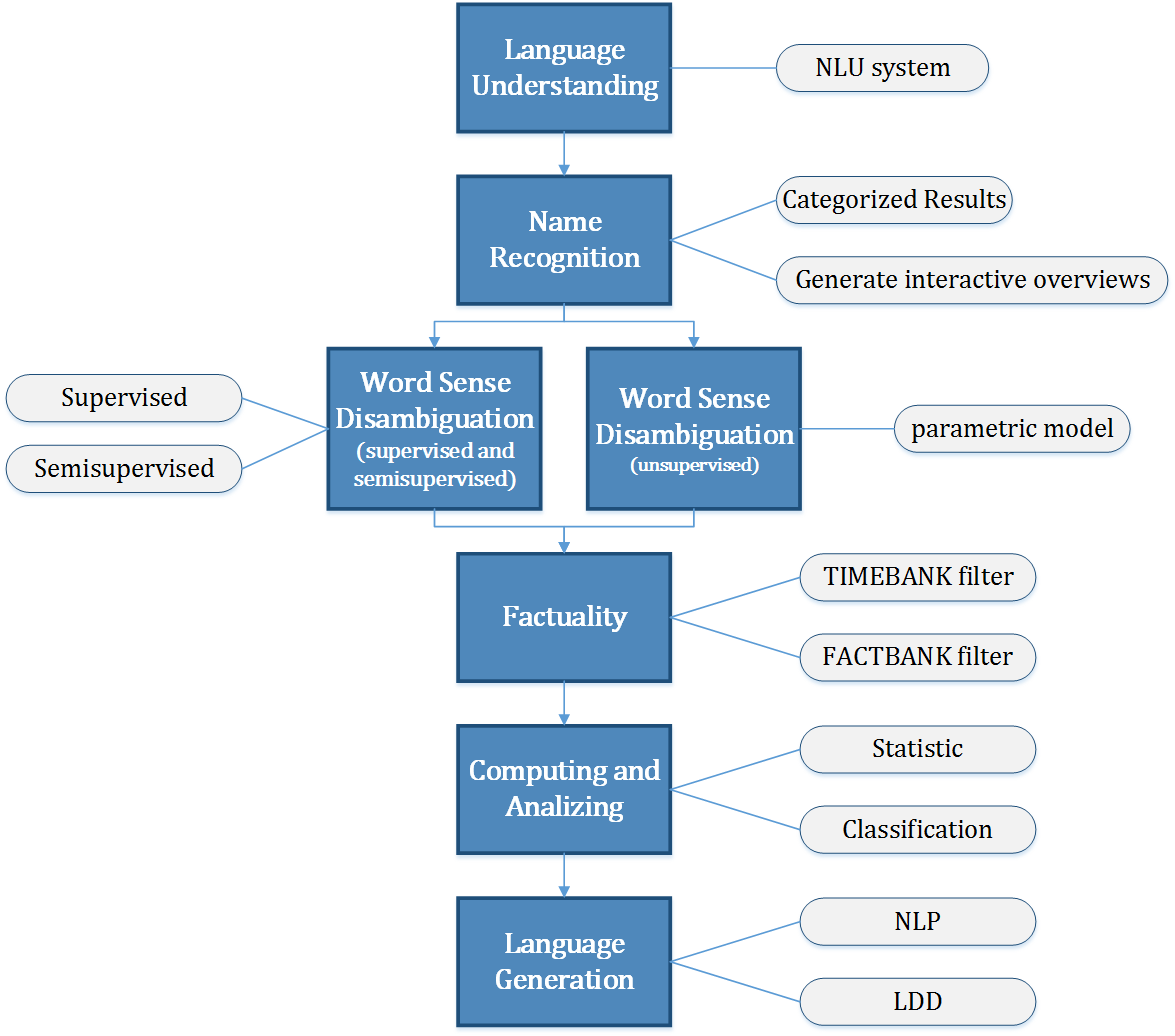
\includegraphics[width=1.8\columnwidth]{Union_Background_Chart_1}
	\end{center}
	\caption{The process of metadata creation.}
\end{figure*}

\subsubsection*{Language understanding}

Natural language understanding (NLU) is a subtopic of natural language processing in artificial intelligence that deals with machine reading comprehension, it's considered an AI-hard problem.

For a machine to understand language, it first has to develop a mental map of words, their meanings and interactions with other words. It needs to build a dictionary of words, and understand where they stand semantically and contextually, compared to other words in their dictionary. To achieve this, each word is mapped to a set of numbers in a high-dimensional space, which are called “word embeddings”. Similar words are close to each other in this number space, and dissimilar words are far apart. Some word embeddings encode mathematical properties such as addition and subtraction.

After the machine has learned word embeddings, the next problem to tackle is the ability to string words together appropriately in small, grammatically correct sentences which make sense. This is called language modeling. Language modeling is one part of quantifying how well the machine understands language.

For example, given a sentence “I am eating pasta for lunch.”, and a word “cars”, if the machine can tell you with high confidence whether or not the word is relevant to the sentence “cars” is related to this sentence with a probability 0.01 and I am pretty confident about it, then that indicates that the machine understands something about words and contexts.

An even simpler metric is to predict the next word in the sentence. Given a sentence, for each word in its dictionary the machine assigns a probability of the word’s likeliness to appear next in the sentence. For example: “I am eating (     ).” To fill in the blank, a good language model would likely give higher probabilities to all edibles like “pasta”, “apple”, or “chocolate”, and it would give lower probability to other words in the dictionary which are contextually irrelevant like “taxi”, “building”, or “music”.

When users search for a sentence, how does the program understand the certain inputs of text? We could build a natural language understanding (NLU) system, in which the system's rules for semantic interpretation are learnt automatically from training data, which uses a set of possible yes-no questions that can be applied to data items.
After that, it follows rules for selecting the best questions at any node on the basis of training data by using a method for pruning trees to prevent over-training.

\subsubsection*{Name Recognition}

If users search for the word "Turkey", the results could be a country or an animal. 
The meaning is totally different and definitely make users very confused if he or she is not very familiar with the word "Turkey". 

There are a lot of misunderstandings like this if users search some words which have multiply meanings. 
Sometimes, the results are fully unrelated and this situation is always annoying. 
That would be troublesome when we count frequency of certain words to rank them.

Therefore, it is significantly crucial for a program to totally understand what users want by name recognition in natural language processing, finally they can find out the results much quicker and will not be confused anymore.

The method to improve the problem above is "categorize the words based on different subjects, topic, or genres" by using online database and python program. 
Metadata is limited in digital libraries and web resources, try to enlarge them with meaningful, organized and desired categories \cite{Kules2006}.

Besides dealing with mutiple-meaning words, the most important part of name recognition is to recognize the special names and terms such as locations, people name, country, even company names and academic terms.
Therefore, it is better for search engine to know what user want and huge name corpus are necessary. 
Plus, this work also can assist previous work.

With above effort, users' exploration and overviews of information could be better supported. It will be very convenient to find the results we want and lower the possibility of misunderstandings if users are not very familiar with finding the appropriate result in specific fields.
\cite{TunThuraThet2010} Users don't need to filter the results which are ranked by browsing frequency popularity but can just obtain the information and relevance by clicking the specific categories and some reasonable choices.

Plus, creating some choices for users is also vital because this make the searching much more oragnized. 
For example, if there are a lot of subtitles such as abstract, introduction, method, or references in some standard research articles, try to make some choices so that the users can easily find out what they want. 
There are a lot of different standard articles in the world.
 Making a suitable choices if someone want to creat a personalzed search engine and interface. 

Also, users are able to choose multiply fields if the results include a lot of relevant fields. 
That's a big motivation for people to handle these problems. 

A lot of online services have done similar tasks before. 
Thus, creating and using an online databases or automated metadata creation are to be recommended. 
The reason is there are many advantages, including integrating with the other cloud services or scaling with what users need such as how to categorize the categories. 
It is beneficial for people who would like to create a convenient and personalized database or metadata.\\\\\\


\subsubsection*{Part-of-speech}

In the English language, we can consider words as the smallest elements that have distinctive meanings. 
Based on their uses and functions, words are categorized into several parts of speech, and the 8 major parts of speech in English grammar are: noun, pronoun, verb, adverb, adjective, conjunction, preposition, and interjection.

\begin{itemize}
	\item Noun (names)\\
	A word or lexical item denoting any abstract (abstract noun: e.g. home) or concrete entity (concrete noun: e.g. house); a person (doctor, Jim), place (farm, Taiwan), thing (earring, refrigerator), idea (happiness), or quality (ambition). 
	Nouns can also be classified as counted nouns or non-counted nouns; some can belong to any category. 
	The most common part of the speech; they are called naming words.
	
	\item Pronoun (replaces)\\
	A substitute for a noun or noun phrase (e.g. them, he). Pronouns make sentences shorter and clearer since they replace nouns.
	
	\item Adjective (describes, limits)\\
	A modifier of a noun or pronoun (big, brave). 
	Adjectives make the meaning of another word (noun) more precisely.
	
	\item Verb (states action or being)\\
	A word denote an action (walk), occurrence (happen), or state of being (be).
	Without a verb, a group of words cannot be a clause or sentence.
	\item Adverb (describes, limits)\\
	A modifier of an adjective, verb, or other adverb (very, quite). 
	Adverbs make your writing more precisely.
	
	\item Preposition (relates)\\
	A word that relates words to each other in a phrase or a sentence and aids in syntactic context (in, of). 
	Prepositions show the relationship between a noun or a pronoun with another word in a sentence.
	
	\item Conjunction (connects)\\
	A syntactic connector; links words, phrases, or clauses (and, but). 
	Conjunctions connect words or group of words.
	
	\item Interjection (expresses feelings and emotions)\\
	An emotional greeting or exclamation (Huzzah, Alas). 
	Interjections express strong feelings and emotions.
\end{itemize}

\subsubsection*{Part-of-speech tagging}

Part of speech tagging (POS tagging), also called grammatical tagging or word-category disambiguation, which is a process of assigning a part of speech to each word in a sentence that based on both definition and its context.\\

\subsubsection*{Word sense disambiguation: supervised and semi-supervised approach}

Word sense disambiguation (WSD) is an open problem of natural language processing and ontology. 
WSD identifies which sense of a word (i.e. meaning) is used in a sentence, when the word has multiple meanings \cite{Du2013}. 

\begin{figure}[tbh]
	\begin{center}
		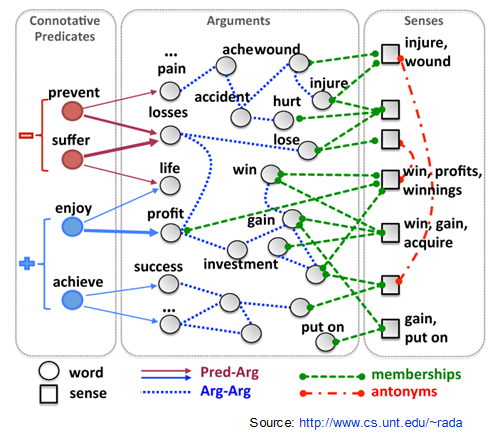
\includegraphics[width=\columnwidth]{Union_Background_Chart_WSD}
	\end{center}
	\caption{GWord+Sense with words and senses. \label{fig1}}
\end{figure}

The solution to this problem impacts other computer-related writing, such as discourse, improving relevance of search engines, anaphora resolution, coherence, inference et cetera.

Word Sense Disambiguation (WSD) is related to natural language processing and is also linked with computational languages. 
People introduced it as a solution when they felt the need of some complex problems like machine translation, information retrieval, speech processing and text processing ,etc. 

WSD is mainly focused on determining the sense of word, computationally which is used in a problem by using that word in a particular context. 
Inspite of having a greater number of existing disambiguation algorithms, WSD still has an open problem with the three main parts of the WSD methods being considered by literature: Supervised, Unsupervised and semi-supervised. 

The human brain is quite proficient at word-sense disambiguation. 
The fact that natural language is formed in a way that requires so much of a reflection of that neurological reality. 
In other words, human language developed in a way that reflects (and also has helped to shape) the innate ability provided by the brain's neural networks. 

In computer science and the information technology that is enable, it has been a long-term challenge to develop the ability in computers to do natural language processing and machine learning. 

\subsection*{Supervised}

Supervised methods are based on the assumption that the context can provide enough evidence on its own to disambiguate words. Probably every machine learning algorithm going has been applied to WSD including associated techniques, such as feature selection, parameter optimization, and ensemble learning.

\begin{figure}[tbh]
	\begin{center}
		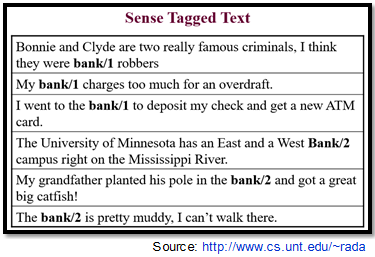
\includegraphics[width=\columnwidth]{Union_Background_Chart_sup1}
	\end{center}
	\caption{Sense tagged text.}
\end{figure}
\begin{figure}[tbh]
	\begin{center}
		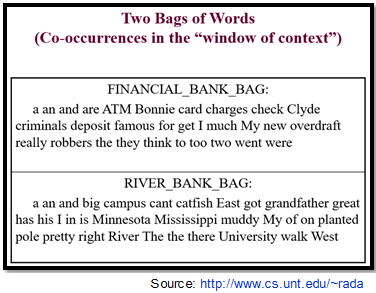
\includegraphics[width=\columnwidth]{Union_Background_Chart_sup2}
	\end{center}
	\caption{Two bags of words(bank).}
\end{figure}
\begin{figure}[tbh]
	\begin{center}
		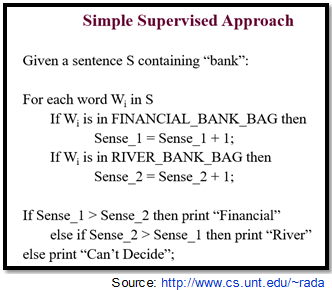
\includegraphics[width=\columnwidth]{Union_Background_Chart_sup3}
	\end{center}
	\caption{Simple Supervised approach.}
\end{figure}

Support Vector Machines and memory-based learning have been shown to be the most successful approaches to date, probably because they can cope with the high-dimensionality of the feature space. 

However, these supervised methods are subject to a new knowledge acquisition bottleneck since they rely on substantial amounts of manually sense-tagged corpora for training, which are laborious and expensive to create \cite{aramossoto2016onthe}.

\subsubsection*{Semi-supervised}

Because of the lack of training data, many word sense disambiguation algorithms use semi-supervised learning, which allows both labeled and unlabeled data. 
The Yarowsky algorithm was an early example of such an algorithm \cite{Gartner201317}. It uses the 'One sense per collocation' and the 'One sense per discourse' properties of human languages for word sense disambiguation. 
Based on observation it has been shown that words tend to exhibit only one sense in most given discourse and in a given collocation. \cite{5599823}

\begin{figure}[tbh]
	\begin{center}
		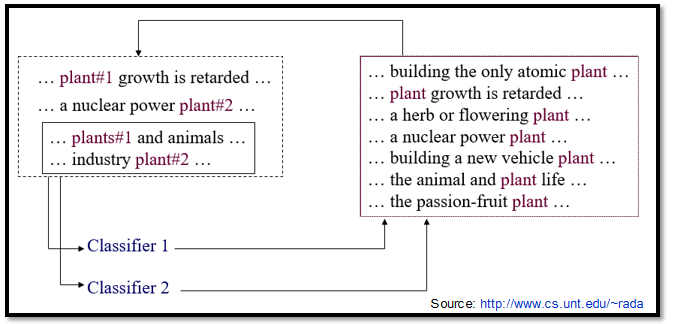
\includegraphics[width=\columnwidth]{Union_Background_Chart_semi}
	\end{center}
	\caption{Classifier that improves over the basic classifier. \label{fig3}}
\end{figure}

The bootstrapping approach starts from a small amount of seed data for each word: either manually tagged training examples or a small number of surefire decision rules. 
The seeds are used to train an initial classifier, using any supervised method. 
This classifier is then used on the untagged portion of the corpus to extract a larger training set, in which only the most confident classifications are included. 
The process repeats, each new classifier being trained on a successively larger training corpus, until the whole corpus is consumed or a given maximum number of iterations is reached \cite{Blascheck2016}.

Other semi-supervised techniques use large quantities of untagged corpora to provide co-occurrence information that supplys the tagged corpora. 
These techniques have the potential to help in the adaptation of supervised models to different domains.

Also, an ambiguous word in one language is often translated into different words in a second language depending on the sense of the word. 
Word-aligned bilingual corpora have been used to infer cross-lingual sense distinctions, a kind of semi-supervised system.\cite{Cheslow2014}

\subsubsection*{Unsupervised}
Unsupervised WSD is the third part of Word sense disambiguation, it has to focus in the sense of the word which is being used in a sentence. 
Unsupervised WSD, which rely on single writing can be approached by the use of Naive Bayes' model, which mainly focuses on unsupervised part of the context. 
In this model,we will know that a number of sentences are used which contains a particular word which has several meanings. 
The main goal of this model is to divide those words into a specified number of sense groups \cite{4028513}. 
The Naive Bayes model applied mathematically entirely focuses on the issue of feature selection, which describes its two types:

\begin{enumerate}
	\item Pedersen and Bruce local type features.
	\item WordNet-based feature selection.
\end{enumerate}

Three different feature sets have been used by 'Pedersen and Bruce' (under Naive Bayes model) for each word to formulate such a model describing the distributions of sense groups of that word in Unsupervised WSD.

Features which were taken into account are:
\textbf{Morphology:} The pattern of word formation in a particular language is called as Morphology. 
This feature represents the morphology \cite{5494927} of the ambiguous word and is denoted by M. 
In case of nouns, M acts as Binary which indicates whether the word is plural or singular. 
For verbs, M indicates the tense of the verb and can have up to seven possible values.But this feature is not applicable for adjectives.

\textbf{Part-of-speech:} This feature represents the part-of-speech \cite{6982457} of the word and tells the position of the ambiguous word. Each POS feature can have one of five possible values: noun, verb, adjective, adverb or other.

\textbf{Co-occurences:} This feature also acts as binary variables representing whether the most frequent content word in all the sentences contain the ambiguous word can occur anywhere in the sentence or not.\\\\

\begin{enumerate}
	\item WordNet-based feature selection:
\end{enumerate}

WordNet is a large lexical database of English. The approach to WSD relies on a set of features formed by the actual words occuring near the target word and reduces the size of this feature set by performing knowledge-based feature selection that relies entirely on WordNet.
The WN semantic network provides the words considered relevant for the set of senses taken into consideration corresponding to the target word.

In WordNet, noun is the most developed portion as per the research done over the performance for knowledge-based disambiguation.
For adjectives, the same disambiguation method has taken into account as the similarity relation, which  is typical of this part of speech.
Verbs are suggested to use additionally whenever possible. 
As a result of using only those words indicated as being relevant and recommended by WordNet, a much small vocabulary was obtained. Therefore, a much smaller number of features were taking part in the disambiguation process.

Therefore, this background focuses mainly on the issues of feature selection for unsupervised WSD performed with an underlying Naive Bayes model.
\todo{Really? This section is shorter.}

The difference between 'Supervised' and 'Unsupervised' WSD is:

\begin{enumerate}
	\item The Supervised WSD approach requires a large amount of data in order to achieve a reliable result and generally the scope is limited to some words. 
	Whereas the Unsupervised WSD approach does not use any corpus and suggests the suitable information extracted to the word knowledge base.
	This method is used in case of performing WSD without data learning.
	\item The Supervised approaches make use of information from labeled training data while the Unsupervised does not depend upon any labeled data, it uses a multi-lingual thesaurus that contains millions of biomedical and health related concepts, their synonymous names and their relationships.
\end{enumerate}

\todo[inline]{A summary on list format can be motivated, but then each item need to be brief and you should not introduce anything new like UMLS in it.}

\subsubsection*{Factuality}

In the process of producing metadata, which should be the most precise information and representing the text, validity of such metadata must be checked. Therefore, tools for fact checks are developed based on linguistic techniques. 

The tool could detect facts and excludes authors' subjective opinions \cite{Agerri2014}. From the authors's perspective, the two main set of tools having such functions is TIMEBANK and FACTBANK. (yes, the authors used capitalized name)

TIMEBANK was first proposed in \cite{pustejovsky2003timebank}. 
The idea was based on that English language has different tenses which could be exploited as signals for fact check. 
An example below could help to clarify the ideas. Let's examine these sentences:

\begin{itemize}
	\item I will go to Chimei museum tomorrow.
	\item Chimei museum is near Tainan District.
	\item I was in UK in 2012.
\end{itemize}

The first sentence is simple future tense which implies something has never actually happened, the second sentence is simple present tense which can directly imply facts, and the last sentence is in simple past tense which is about something already happened (which is facts), but is no longer a fact right now, so such fact must be used with caution. 

The reason for introducing such tool is that even scientific research articles can be glittering with subjective comments, opinions or even assumption from authors \cite{schultze2000confessional}. In addition to TIMEBANK, many other tools can be another filter for fact extraction. \cite{Dave2003mining} Identify words, clauses and phrases that show emotional state of the authors. 

The choice in expression of facts could also be a helpful indicator to show whether authors are subjectively supporting a cause, an opinion and so on \cite{Wiebe2005}. Among these mentioned approaches, this paper highly favors creation a kind of thesaurus compiled of linguistic signaling for non-factually statements such as FACTBANK, which is built by \cite{Sauri2009}. 
Following example shows how subjective statements can be picked out.

\begin{itemize}
	\item Channelization would guarantee high flow velocity in rivers, flooding and consequent degradation of riparian community (1a).
	\item Funding agencies would be happy with big entrepreneurs, instead of small and medium enterprises (1b).
	\item Tolerance to dictatorship would has negative influences on anarchist movement (2a).
	\item Tolerance to dictatorship would doom anarchist movement (2b).
\end{itemize}

It is easy to find in statement (1a) is an absolute fact. 
Statement (1b) is however affected by emotional state of authors. 
After re-writing (1b) into: Funding agencies lend more money with lower interest rate to big entrepreneurs, instead of small 
and medium enterprises,sentence (1b) become a face-based statement. 
In another case, statement (2a) is a fact-based statement while in statement (2b), authors are stressing their dislike toward dictatorship.

Fact checks in language generation is a new field but many useful tools have been developed. Each of them has their own function and could complement each others. In the limit of this study, we are using both of TIMEBANK and FACTBANK together for fact check.


\subsubsection*{Language generation}

Natural language generation (NLG) is one branch of natural language processing. The goal is generating the words that human being uses via machine automatically. In order to use this technique, six basic activities are done: 

\begin{enumerate}
	\item Content determination: In this active, we create some messages which are communicated in the text. 
	These messages shall be labeled and the entity in the messeges is also distinguished, which is convenient for us to 
	use these data within the following step.
	\item Discourse planning: This part is closely related to the previous part. 
	We determine the order and the structure of the messeges.
	\item Sentence aggregation:This part combines several messeges into sentences. 
	Although some of messeges have been a sentence, we can improve the influency of messeges by combining them.
	\item Lexicalization: This part make the messege more precise by use the specific words and concepts. 
	Then people can get the ideas of the messeges more quickly.
	\item Referring expression generation: This part is a litte same as the previous part. 
	But the difference is that this part differentiate the one domain to the other domains.
	\item Linguistic realization: Last part is to make the expression follow the rules of grammer, part of speech and the natural language rule.
	
\end{enumerate}
\cite{aramossoto2016onthe}. The advantage of this technique is that it is flexible, since there is no standardization. But it also has the difficulty in the implication of this technique. \cite{aramossoto2016onthe} No standardization means that no rules can be followed. 

Without logic method, it is almost impossible to code and be realized by computer. 
Thus, the another concept is proposed. 
This way has the logical method, also the algorithm is easy to realize. 
The technique is linguistic discription of data.
\todo{Now you jump too far. More explanations are needed.}
Linguistic description of data (LDD) is a concept that applied the fuzzy set theory in the linguistic field. 
At the beginning, comparing to the NLG field, it is a newer technique to solve the problem of language generation. 
However, the basic steps of LDD have been built. 
The four main parts in this technique are inputing data, linguistic variable, fuzzy quantifiers and evaluation criteria \cite{aramossoto2016onthe}. 
Some of them are similar to the concept. 
The advantage of this technique is that it has been implied in many fields just like weather forecast \cite{Ramos-SotoBBT14}. 
Also, many practical methods have been proposed. However, it still has a long way to go.

These two techniques are usually combined together nowadays. 
The concept of NLG and the practical approach of LDD could be used in the same time to provide the better performance in language generate field.
\subsection{API and search engine}
An API is short-hand of  application programming interface, which include components to define a process of communication and data processing on computer. 
It is necessary to create a search engine as we mentioned at the beginning of this report.
A good example of API is HAPI on Python. 
According to \cite{Kochanov201615}, HAPI is a library included in Python. 
As the library has a collection of defined process, it allow users and other parties (which could be robots or others users at other ends) to interact with each other.
Main functions of the HAPI have been including sending uploads, data filtration and other manipulation. 
The outcomes of such process can be formatted with variable forms. 
As described by \cite{Hedbrant20162206}, programming interface can include following systems:
\begin{itemize}
	\item SOAP: Simple Object Access Protocol
	\item REST: Representational State Transfer
	\item UDDI: Universal Description, Discovery, and Integration
	\item WSDL: Web Service Definition Language
\end{itemize}
	Other programing system can be included as well. 
	SOAP is among a field attracting many recent researches. 
	A good review about SOAP could be found from the work of \cite{Hsieh2009424}. 
	SOAP has important roles in field monitoring as handling a huge amount of data can be trouble some in many senses. 
	SOAP in conjunction with other programming techniques, such as distributed computing, are employed because it can solve 3 problems listed below:
	\begin{itemize}
		\item Is the system scalable: 
		There are systems that suitable for a fixed amount of data, but not functional when the need of expending data storage comes in place. 
		With such system, programmers will have to build another system. 
		That would be a waste of human resource, time and money.
		\item Is the system reliable: 
		In other words, can data be stored safely. 
		Many data obtained in field monitoring are expensive. 
		Therefore, it is important to make sure data will be always there whenever a need of retrieval arisen. 
		Also, the data may be retrieved, processed and formatted by many people involved in the system.
		A reliable system will not be broken down easily and foremost, data will be safely stored.
		\item Is the system accessible: 
		This matter can be put in two questions 1- When we need to use the data, is it hard to retrieve it from the system. 
		Do we need trained personal to do that job.
		And if we do, which level of training is necessary. 
		2- How many people can access the system. 
		
	\end{itemize}
	It is proven in many engineering projects, the application of SOAP can help overcome these problems, especially in term of increasing accessiblity.
	\subsubsection{Search engine}
	As mentioned above, creating a search engine is an example of API application. 
	In this section we feel the need to give an example of how to create search engine with API. 
	We found an inspirational example from the work of \cite{Noei2016135}. 
	Although the authors not just using SOAP, but also more advanced Object Access Protocol such as Java, it shows that OAP in general improve code and design. 
	Consequently, it saves time and effort in developing new program.
	The authors also offer EXAF (EXample Applications Finder) so that program developers can find other examples that fits their interest.
	
\newpage % Ends the current page and causes all figures and tables to be printed